\documentclass[10pt]{article}
\usepackage[margin=0.55in]{geometry}
\usepackage{amsmath, amssymb}
\usepackage{enumitem}
\usepackage{titlesec}
\usepackage{tikz}
\usetikzlibrary{patterns, arrows.meta}
\usepackage{wrapfig}
\setlist{nosep, leftmargin=1.2em}
\titlespacing*{\section}{0pt}{4pt}{2pt}
\titleformat{\section}{\normalsize\bfseries}{}{0pt}{}
\setlength{\parskip}{3pt}
\setlength{\parindent}{0pt}
\pagestyle{empty}

\begin{document}

\begin{center}{\large\bfseries Perfect Punching --- Physics White Paper}\end{center}

\section*{The problem}
A two-way concrete plate slab bears on columns. At each column two demands act at the slab--column interface: direct shear $V_u$ (vertical reaction) and an \textbf{unbalanced moment} $M_u$ (the moment the slab cannot distribute evenly between opposite column strips). $M_u$ arises whenever spans, loads, or stiffnesses are asymmetric across a column.

\section*{Moment transfer split (ACI 318 \S8.4.2.3)}

\begin{wrapfigure}{r}{0.46\textwidth}
\vspace{-18pt}
\centering
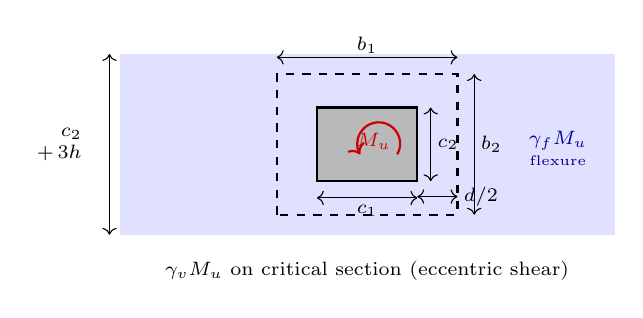
\begin{tikzpicture}[scale=0.85, every node/.style={font=\scriptsize}]
  % effective flexure strip (c2 + 3h), horizontal band
  \fill[blue!12] (-3.7, -1.35) rectangle (3.7, 1.35);
  % critical section (d/2 offset from column face)
  \draw[dashed, thick] (-1.35, -1.05) rectangle (1.35, 1.05);
  % column
  \fill[gray!55] (-0.75, -0.55) rectangle (0.75, 0.55);
  \draw[thick] (-0.75, -0.55) rectangle (0.75, 0.55);
  % unbalanced moment arrow on column (curved)
  \draw[->, thick, red!80!black] (0.45,-0.15) arc[start angle=-30, end angle=210, radius=0.32];
  \node[red!80!black] at (0.1, 0.05) {$M_u$};
  % column dimension labels
  \draw[<->] (-0.75, -0.8) -- (0.75, -0.8) node[midway, below=-1pt] {$c_1$};
  \draw[<->] (0.95, -0.55) -- (0.95, 0.55) node[midway, right=-1pt] {$c_2$};
  % critical section dimensions
  \draw[<->] (-1.35, 1.3) -- (1.35, 1.3) node[midway, above=-2pt] {$b_1$};
  \draw[<->] (1.6, -1.05) -- (1.6, 1.05) node[midway, right=-1pt] {$b_2$};
  % d/2 annotation
  \draw[<->] (0.75, -0.78) -- (1.35, -0.78);
  \node at (1.7, -0.78) {$d/2$};
  % strip width label
  \draw[<->] (-3.85, -1.35) -- (-3.85, 1.35);
  \node[align=right] at (-4.6, 0) {$c_2$\\$+\,3h$};
  % flexure label
  \node[blue!55!black] at (2.85, 0.05) {\textbf{$\gamma_f M_u$}};
  \node[blue!55!black, font=\tiny] at (2.85, -0.25) {flexure};
  % shear eccentricity label
  \node[below=6pt] at (0, -1.35) {\textbf{$\gamma_v M_u$} on critical section (eccentric shear)};
\end{tikzpicture}
\vspace{-8pt}
\end{wrapfigure}

\vspace{-6pt}
\[
M_u = \underbrace{\gamma_f M_u}_{M_f,\ \text{flexure}} + \underbrace{\gamma_v M_u}_{M_v,\ \text{shear ecc.}}
\]
\vspace{-16pt}
\[
\gamma_f = \frac{1}{1 + \tfrac{2}{3}\sqrt{b_1/b_2}}, \quad \gamma_v = 1 - \gamma_f
\]
$\gamma_f$ (\emph{gamma-f}, flexure-transfer fraction) and $\gamma_v$ (\emph{gamma-v}, shear-eccentricity fraction) sum to one. $M_f$ is resisted by flexure across an effective strip of width $c_2 + 3h$ centered on the column. $M_v$ is resisted by eccentric shear around the critical section offset $d/2$ from the column face ($b_1, b_2$ = critical-section dimensions parallel and perpendicular to the moment span). $M_v$ is what makes punching a two-way shear problem.

\section*{Critical section}
Perimeter $b_0$ closes for interior columns but \textbf{truncates} at slab edges, reentrant corners, and openings within $4h$ (\S22.6.4.3). Perimeter length and centroid shift accordingly --- which is why 3D B-rep geometry is required.

\section*{Combined shear stress}
\vspace{-10pt}
\[
v_u(\theta) = \frac{V_u}{b_0\, d} \pm \frac{\gamma_v\, M_u\, c}{J_c}
\]
$\theta$ (\emph{theta}) = angle around the critical-section perimeter; $c$ = distance from the section centroid to the point; $J_c$ = polar moment of inertia of the section about its centroid (\S R8.4.4.2.3). $v_u$ peaks at the face farthest from the centroid in the direction of $M_u$; edge/corner columns shift the centroid away from the free edge, amplifying the peak.

\section*{Capacity (\S22.6.5.2)}
\vspace{-10pt}
\[
\phi v_c = \phi\, \lambda_s\, \lambda\, \min\!\left(\, 4\sqrt{f'_c},\ \bigl(2+\tfrac{4}{\beta}\bigr)\sqrt{f'_c},\ \bigl(\alpha_s \tfrac{d}{b_0}+2\bigr)\sqrt{f'_c}\,\right) \ \text{[psi]}
\]
$\phi$ (\emph{phi}) = strength-reduction factor; $\lambda$ (\emph{lambda}) = lightweight-concrete factor; $\lambda_s$ (\emph{lambda-s}) = size-effect factor; $\beta$ (\emph{beta}) = long/short column ratio; $\alpha_s$ (\emph{alpha-s}) = 40/30/20 (interior/edge/corner). DCR = $v_{u,\max}/\phi v_c$; governs when $>1.0$.

\section*{What Perfect Punching computes}
Geometry $\to$ plate-bending analysis for $V_u, M_u$ per column (EFM regular, FEA general) $\to$ critical-section shell offset from column face and truncated by slab B-rep via opencascade.js $\to$ exact $b_0, c, J_c$ $\to$ $v_u(\theta)$ gradient on the section surface $\to$ $\phi v_c$ $\to$ DCR color-coded in the 3D viewport.

\section*{Why the geometry kernel matters}
$b_0$, $c$, and $J_c$ are integrals over the critical-section surface. For truncated sections those integrals run on a Boolean result. Mesh CSG gives numerically wrong perimeters and centroids at reentrant corners and sliver edges --- exactly where punching governs. OCCT exact B-rep makes the capacity check as accurate as the code equation allows.

\vspace{2pt}\hrule\vspace{2pt}
{\scriptsize ACI 318-19 Ch.~22 \S\S 8.4.2, 22.6 \,\textbar\, MacGregor \& Wight, \emph{Reinforced Concrete}, Ch.~13 \,\textbar\, Nilson et al., \emph{Design of Concrete Structures}, Ch.~13.}

\end{document}
